%\title{ABNIT data structures and their theoretical justifications.}

%\documentstyle{article}
\documentclass{article}
%\usepackage[dvips]{graphicx}
\usepackage{graphicx}

\title{Representation and conversion of the set of wavefunctions\\
       {\normalsize{(X. Gonze, Y. Suzukawa, M. Mikami)}}}
\begin{document}
\maketitle

\section{The block of wavefunctions for one ${\bf k}$-point and one
spin-polarization}
\label{sec:A1}
\hspace*{\parindent}
\vskip 1em
* We will now consider a wavefunction as an object made of
{\tt 2*npw\_k*nspinor} double precision numbers, whose signification
and use will \underline{not} be described here.

\vskip 1em
* {\tt npw\_k} is an integer number, that may vary from ${\bf k}$-point
to ${\bf k}$-point, while nspinor will be 1 or 2, and will
\underline{not} vary in the set of wavefunction.

\vskip 1em
* A block of wavefunction is made of {\tt nband\_k} wavefunctions,
considered for one specific ${\bf k}$-point and spin-polarization.
The number of double precision coefficients in a block of WFs is
{\tt 2*npw\_k*nspinor*nband\_k}.

\vskip 1em
* The set of wavefunctions is made of all the blocks for different
${\bf k}$-points and spin-polarizations. The number of spin-polarization,
{\tt nsppol}, can be 1 or 2. Note that {\tt nsppol}=2 and
{\tt nspinor} = 2 are mutually exclusive. \\
The number of ${\bf k}$-points, {\tt nkpt} can be as small as 1, but
can also be a large number, bigger than 1000. There must be the same number
of ${\bf k}$-points for both spin-polarizations.

\vskip 1em
* As {\tt npw\_k} and {\tt nband\_k} can vary with the ${\bf k}$-point
(and polarization for {\tt nband\_k}), we have arrays
\begin{eqnarray*}
{\tt npwarr(1:nkpt,1)}&\longrightarrow & {\tt npw\_k = npwarr(ikpt,1)} \\
{\tt nband(1:nkpt*nsppol)}&\longrightarrow & {\tt  nband\_k =
nband(ikpt+(isppol-1)*nkpt)}
\end{eqnarray*}

\vskip 1em
\section{Eigenvalues and occupation numbers}
\label{sec:B1}
\hspace*{\parindent}
\vskip 1em
* At each ${\bf k}$-point and spin-polarization, there is also a set of
eigenvalues and a set of occupation numbers, in the Ground-State case
({\tt formeig} = 0) ; \\
\hspace*{15ex} {\tt eig\_k(1:nband\_k)} \\
\hspace*{15ex} {\tt occ\_k(1:nband\_k)} \\
and, in the Response-Function case ({\tt formeig} = 1), a complex matrix
of eigenvalues \\
\hspace*{15ex} {\tt eig\_k(1:2*nband\_k**2)}

\section{Storage of wavefunctions : disk file}
\label{sec:C1}
\vskip 1em
\hspace*{\parindent}
The disk files are made of a header, followed by the blocks of
wavefunctions, eigenvalues (and occupation numbers, in the ground-state
case) for each ${\bf k}$-point and spin-polarization, then some information
on the history of atomic positions and forces. \\
The part related to the wavefunctions block is written as follows :

\noindent
{\tt
do isppol= 1, nsppol \\
\, do ikpt = 1, nkpt \\
\, \, write(unit) npw\_k*nspinor, nband\_k \\
\, \, if(formeig = = 0) then \\
\, \, \, write(unit) eig\_k(1:nband\_k), occ\_k(1:nband\_k) \\
\, \, end if \\
\, \, do iband = 1, nband\_k \\
\, \, \, if(formeig = = 1) then \\
\, \, \, \, write(unit) eig\_k(1:2*nband\_k) \\
\, \, \, end if \\
\, \, \, write(unit) wavef\_k(1:2, 1:npw\_k*nspinor, iband) \\
\, \, enddo ! iband \\
\, enddo ! ikpt \\
enddo ! isppol}

where : \\
* {\tt formeig} = 0 for ground-state {\tt wfs}, and = 1
for response function \\
* {\tt npw\_k, nband\_k, eig\_k, occ\_k, wavef\_k} are related to one
${\bf k}$-point and spin-polarization, and vary with them (this is not
shown explicitly in the above description).

\section{Storage of wavefunctions : core memory (sequential case)}
\label{sec:D1}
\hspace*{\parindent}
\vskip 1em
* In order to describe the storage of wavefunctions, we adopt the same
convention on the meaning of
{\tt npw\_k, nband\_k, eig\_k, occ\_k} and {\tt wavef\_k}.

We have to distinguish two cases : either the full set of wave
function is kept in memory ({\tt mkmem = nkpt}), or only one block
of wavefunction is kept in memory ({\tt mkmem = 0}). The intermediate case,
were a subset of the wavefunctions would be kept in core memory, has
no advantage with respect to one or the other, and has not been allowed.

\label{sec:D2}
\vskip 1em
* If {\tt mkmem = nkpt}, the wavefunctions are kept in the array
{\tt cg}, declared as \\
{\tt
double precision :: cg(2,mpw*nspinor*mband*mkmem*nsppol)
}\\
where {\tt mpw} is the maximum number of plane waves for all ${\bf k}$
points \\
{\tt mband} is the maximum number of bands for all ${\bf k}$ points.

The detailed storage is : \\
\noindent
{\tt
icg = 0 \\
do isppol = 1, nsppol \\
\, do ikpt = 1, nkpt \\
\, \, do iband = 1, nband\_k \\
\, \, \, do ipwsp = 1, npw\_k*nspinor \\
\, \, \, \, index = ipwsp + (iband - 1) * npw\_k * nspinor \\
\, \, \, \, cg(1:2, index + icg) = wavef\_k(1:2, ipwsp, iband) \\
\, \, \, enddo \\
\, \, enddo \\
\, \, icg = icg + npw\_k * nspinor * nband\_k \\
\, enddo \\
enddo
}

\vskip 1em
* If {\tt mkmem} = 0, the wavefunctions are kept on disk, and the block
of wavefunctions related to one ${\bf k}$-point and spin-polarization is
read in the array {\tt cg\_disk}, declared as \\
{\tt double precision :: cg\_disk (2, npw\_k * nspinor * nband\_k)}\\
reallocated for each block, with the correct dimensions.

The self-consistent update of wavefunctions will actually involve
\underline{two} disk files. During one ``step'' of the SCF procedure,
the ``old'' wavefunctions are contained in a first disk file, that is
read block of wavefunctions by block of wavefunctions, while the
``new'' wavefunctions are written on another disk file :
%[CAUTION: how to realize the figure ??]
%\begin{figure}[h]
%\giffile[\pbmfat(3cm, 5cm){test}]
%{file=sr8000.gif,width=5cm, height=3cm}
%\end{figure}

\begin{figure}[h]
\begin{center}
%\includegraphics[width=5cm,clip]{YOS}
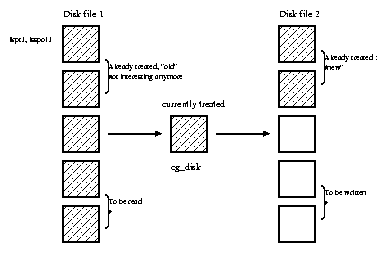
\includegraphics[width=10cm,clip]{Figure}
%\epsfbox{YOS} % error !
\end{center}
\end{figure}

\label{sec:D3}
\vskip 1em
* Independently of the value of {\tt mkmem}, the eigenvalue and
occupation numbers are kept in core memory. \\
For the occupation numbers, one has the array occ \\
{\tt double precision :: occ (mband * nkpt * nsppol)}\\
with detailed storage\\
{\tt
bantot = 0 \\
do isppol = 1, nsppol \\
\, do ikpt = 1, nkpt \\
\, \, occ (1 + bantot : nband\_k + bantot) = occ\_k (1:nband\_k) \\
\, \, bantot = bantot + nband\_k \\
\, enddo \\
enddo}

\vskip 1em
* The storage of eigenvalues, in the ground-state case ({\tt formeig} = 0)
is perfectly identical to the one of occupation numbers, in the array
eigen :\\
{\tt double precision :: eigen (mband * nkpt * nsppol)}\\
For the response-function case, we have matrices of eigenvalues :\\
{\tt double precision :: eigen (2 * mband **2 * nkpt * nsppol)}\\
{\tt
ban2tot = 0 \\
do isppol = 1, nsppol \\
\, do ikpt = 1, nkpt \\
\, \, eigen(1+ban2tot: 2*nband\_k**2 + ban2tot) = eig\_k(1:2*nband\_k**2) \\
\, \, ban2tot = ban2tot + 2*nband\_k**2 \\
\, enddo \\
enddo}

\section{Storage of wavefunctions : core memory (parallel case)}
\label{sec:E1}
\hspace*{\parindent}
\vskip 1em
* In the parallel case, the storage of wavefunctions is spread on the
different processors, while all processors have a copy of the arrays
{\tt eigen} and {\tt occ}, whose storage is \underline{not} modified
compared to the sequential case. We will thus focus on the wavefunctions.

\vskip 1em
* The fundamental question is : does the present processor treat this
${\bf k}$-point and spin-polarization ? If yes, the corresponding block
will be in core memory. If no, it will not. In the parallel case, it
might be interesting to have {\tt mkmem} lower than {\tt nkpt},
as soon as the number of ${\bf k}$ points to be treated by a processor
is lower or equal to {\tt mkmem}. We still have the array {\tt cg}
declared as \\
{\tt double precision :: cg(2, mpw * nspinor * mband * mkmem * nsppol)}\\
with detailed storage :\\
{\tt
icg = 0 \\
do isppol = 1, nsppol \\
\, do ikpt = 1, nkpt \\
\, \, if (``(ikpt, isppol) not treated by the present processor'') cycle \\
\, \, do iband = 1, nband\_k \\
\, \, \, do ipwsp = 1, npw\_k * nspinor \\
\, \, \, \, index = ipwsp + (iband-1) * npw\_k * nspinor \\
\, \, \, \, cg (1:2,index + icg) = wavef\_k (1:2, ipwsp, iband) \\
\, \, \, enddo \\
\, \, enddo \\
\, \, icg = icg + npw\_k * nspinor * nband\_k \\
\, enddo \\
enddo}

\label{sec:E2}
\vskip 1em
* Let us specify the meaning of ``({\tt ikpt,isppol}) not treated by the
present processor'' \\
There are two parallel modes. Either the parallelism is done with
respect to ${\bf k}$-points only, or it is allowed with respect to
${\bf k}$-points \underline{and} bands. In the present status of ABINIT (v3.2),
in the ground-state case, the parallelism is done only with respect to
${\bf k}$-points, while in the response-function case, it is done with
respect to ${\bf k}$-points and bands. The user has no control yet on
this choice.

\vskip 1em
* The case {\tt paralbd} = 0 (no parallelism over the bands) \\
(Warning : Should be updated ! similar to the case {\tt paralbd} = 1 in v3.2).
The attribution of a ${\bf k}$-point for some spin-polarization is
computed in the routine {\tt distrb.f}, and generates an array
{\tt kpt\_distrib(1:nkpt)} giving for each ${\bf k}$-point, the number
of the processor that treats it.
This number, for each processor, is obtained through a call to the MPI
routine MPI\_COMM\_RANK, and stored in the variable {\tt me}.
The condition for this ${\bf k}$-point {\tt ikpt} to be treated by the
processor $me$ is thus :\\
{\tt if (kpt\_distrb(ikpt) == me)} then ...

\label{sec:E3}
\vskip 1em
* The case {\tt paralbd = 1} (parallelism over bands is allowed)\\
In this case, some bands of a same ${\bf k}$-point can be treated by
different processors. However, for different reasons, the processors
that treat bands belonging to a ${\bf k}$-point need to know
\underline{all} the wavefunctions of this ${\bf k}$-point.
Thus one block of wavefunction for one ${\bf k}$-point will be copied on
different processors.

The attribution of a band of some ${\bf k}$-point, for some
spin-polarization, is computed in the routine {\tt distrb2.f},
and generates an array {\tt proc\_distrb (1:nkpt, 1:mband)} for each
spin-polarization, giving for each ${\bf k}$-point and band, the number
of the processor that treats it.

The condition, for the processor {\tt me}, to contain the block of
wavefunctions associated to the ${\bf k}$-point {\tt ikpt}, is to have
at least one band attributed to it : \\
{\tt if (minval(abs(proc\_distrb(ikpt, 1:nband\_k)-me))=0) then ...}\\
(this is a very condensed F90 formulation !)


\section{Reading and Conversion of wavefunctions : principles
[routine {\tt inwffil.f}] }
\label{sec:F1}
\hspace*{\parindent}
\vskip 1em
* We have seen in the document Data structures 1WF, page \pageref{sec:G1},
how to derive the wavefunction characterized by {\tt nspinor}, {\tt kpt},
{\tt kg}, and {\tt istwfk}, from some other wavefunction with different
parameters. Here, we consider the conversion of blocks of wavefunctions,
for which the additional parameters {\tt nband\_k}, {\tt nkpt} and
{\tt nsppol} are present, and can be varied.

\vskip 1em
* Typically, the starting wavefunctions are on a disk file, and they
must generate other wavefunctions, either in core memory or on another
disk file. The treatment will differ in those two cases, especially
because of the core memory management. In this operation, the goal is
not to use \underline{more} memory than in the rest of the code!
Efficiency is a secondary concern, in the sequential version. It is
more important in the parallel version, however, as we will see later.

\vskip 1em
* Thus, it is \underline{not} possible to create two arrays with
dimensions \\
{\tt cg1 (2, mpw1 * nspinor1 * mband1 * mkmem1 * nsppol1)}\\
{\tt cg2 (2, mpw2 * nspinor2 * mband2 * mkmem2 * nsppol2)}\\
and make the conversion in core memory :

% TEMPORARY ...
\begin{eqnarray}
{\tt disk} \stackrel{\rm rendering}{\longrightarrow}
{\tt cg1} \stackrel{\rm converting}{\longrightarrow}
&{\tt cg2}& \longleftarrow
\mbox{This is not possible !}  \nonumber \\
& \downarrow & \mbox{possibly write} \nonumber \\
& \mbox{disk} &  \nonumber
\end{eqnarray}

\label{sec:F2}
\vskip 1em
* The precise mechanism, with temporary arrays, will depend on the
parameters {\tt mkmem}, the sequential/parallel mode as well as the
relative sizes of the ``input'' and ``output'' blocks of wavefunctions
for each ${\bf k}$-point and spin-polarization. See section
\ref{sec:G1} and \ref{sec:H1}. % and I ??

\vskip 1em
* Independently of this mechanism, we describe the change of
parameters {\tt kpt}, {\tt nband\_k} and {\tt nsppol} now.
Be given an input set of {\tt nkpt1} ${\bf k}$-point wavefunctions,
with ${\bf k}$-points {\tt kpt1(1:3, 1:nkpt1)},
from which the wavefunctions at {\tt nkpt2} ${\bf k}$-points
{\tt kpt2(1:3, 1:nkpt2)} must be deduced.
For each ${\bf k}$-point {\tt ikpt2}, we will find the ${\bf k}$-point
{\tt ikpt1} that allows to generate the closest ${\bf k}$-point, by use
of symmetry operations and translations in reciprocal space, as
explained in Data structures 1WF page \pageref{sec:G2}.
This operation is done in the routine {\tt listkk.f}.

\vskip 1em
* Having assigned one {\tt ikpt1} to each {\tt ikpt2}, we will also have
to select the proper spin-polarization {\tt isppol}.
When {\tt nsppol1} = {\tt nsppol2}, there is no problem, as
{\tt isppol} = 1 goes to {\tt isppol2} = 1, and,
if {\tt nsppol1} = 2, we also have {\tt isppol1} = 2 goes to
{\tt isppol2} = 2.

If {\tt nsppol1} = 1 and {\tt nsppol2} = 2, we will simply use
{\tt isppol1} = 1 for both {\tt isppol2 = 1} and {\tt isppol2 = 2}.
[the conversion from spinor {\tt wf} to spin-polarization {\tt wfs}
is not coded yet]

\label{sec:F3}
If {\tt nsppol1} = 2 and {\tt nsppol2} = 1 (reduction from
spin-polarized to spin-unpolarized), we use {\tt isppol1} = 1 for
{\tt isppol2} = 1. [the conversion from spin-polarized {\tt wfs}
to spinor {\tt wfs} is not coded yet]

\vskip 1em
* The number of bands needs to treated as well. From {\tt nband1\_k}
starting bands, one can generate at most
{\tt nband12 = (nband1\_k/nspinor1) * nspinor2}
output bands, using the mechanism explained in Data structure 1WF, page
\pageref{sec:G1}, if conversion of {\tt nspinor} is needed.

We can have three cases : either \\
\begin{itemize}
\item {\tt nband12 = nband2\_k} In this case, we use all the input
wavefunctions, and generate all the wavefunctions that are needed.
\item {\tt nband12 > nband2\_k} We have too many input bands, for the
restricted number that we need. We actually will read only
{\tt nband12\_min = (nband2\_k/nspinor2) * nspinor} bands.
\item {\tt nband12 < nband2\_k} We do not have enough starting bands.
We will complete the available data either by random numbers (if GS case)
or zeros (if RF case)
\end{itemize}

\vskip 1em
* The conversion of a block of wavefunctions to another block of
wavefunctions is done in the routine {\tt wfconv.f}.

\section{The reading and conversion of wavefunction sets. Sequential
case.}
\label{sec:G1}
\hspace*{\parindent}
\vskip 1em
* We have to distinguish two cases : either the final wavefunctions
must be stored on disk, or they will be in core memory.

\vskip 1em
* Final storage on disk (from disk to disk) [routine {\tt newkpt.f}]
A temporary array, dimensioned so as to be able to contain the biggest
block of wavefunctions of both the input and output files is created :\\
{\tt cg\_disk (2, mpw * mspinor * mband)}

Note that {\tt mband} does not take into account {\tt nband1\_k}, when
it is sufficient to use {\tt nband12\_min}, see page \pageref{sec:F3}.

The blocks {\tt (ikpt2, isppol2)} will be treated in order, while the
blocks {\tt (ikpt1,isppol1)} will be accessed ``randomly'', as needed to
obtain all the {\tt (ikpt2, isppol2)} in turn:
\noindent
{\tt
do isppol2 = 1, nsppol2 \\
\, do ikpt2 = 1, nkpt2 \\
\, \, $\cdot$ select (ikpt1, isppol1) needed for (ikpt2, isppol2) \\
\, \, $\cdot$ read the wavefunction (ikpt1, isppol1) from disks and store them in cg\_disk \\
\, \, $\cdot$ convert the wavefunctions inside cg\_disk to (ikpt2, isppol2) \\
\, \, $\cdot$ write the wavefunctions to disk2 \\
\, enddo \\
enddo
}

\label{sec:G2}
\vskip 1em
* Final storage in core memory (from disk to core, routines
{\tt wfsinp.f} and {\tt newkpt.f})\\
In this case, we have an array \\
{\tt cg2(2, mpw2 * nsoinor2 * mband2 * mkmem2 * nsppol2)}

We will be able to avoid declaring a temporary array {\tt cg\_disk}
only if each of the block of input wavefunctions needs less storage than
each corresponding block in {\tt cg2}, that is
{\tt 2 * npw2\_k * nspinor2 * band2\_k} double precision numbers.
In this case {\tt squeeze} = 0, otherwise {\tt squeeze} = 1.
Unlike the disk to disk case, the order in which the input
wavefunctions are read is not dictated by the need to write the output
wavefunctions in order. On the contrary, we will be able to read each
input wavefunction block only once. The algorithm is as follows :

Step1 (routine {\tt wfsinp.f})

{\tt
do isppol1 = 1, nsppol1 \\
\, do ikpt1 = 1, nkpt1 \\
\, \, if ``(ikpt1, isppol1) is needed to initialize some (ikpt2,isppol2)'' \\
\, \, then \\
\, \, $\cdot$ read (ikpt1, isppol1), store it in \\
\, \, \, cg\_disk if squeeze =1 \\
\, \, \, cg2(ikp2\_stor, isspol2\_stor) if squeeze =0 \\
\, \, do isspol2=1, nsspol2 \\
\, \, \, do ikpt2=1, nkpt2  \\
\, \, \, \, if squeeze = 0, copy from (ikpt2\_stor, isppol2\_stor) to (ikpt2,isspol2) \\
\, \, \, \, if squeeze = 1, copy from cg\_disk to (ikpt2, isppol2) \\
\, \, \, enddo \\
\, \, enddo \\
\, \, else skip (ikpt1, isspol1) \\
\, \, endif \\
\, enddo \\
enddo \\
}

\label{sec:G3}
Step2 (routine {\tt newkpt.f})
{\tt
do isppol2 = 1, nsppol2 \\
\, do ikpt2 = 1, nkpt2 \\
\, \, if squeeze = 0, convert the wavefunctions in block (ikpt2,
isppol2) to their final parameters \\
\, \, if squeeze = 1, do nothing (the conversion already took place in
wfsinp.f) \\
\, enddo \\
enddo}

\section{The reading and conversion of wavefunction sets. Parallel
case}
\label{sec:H1}
\hspace*{\parindent}
\vskip 1em
* In addition to the disk vs core memory choice, we have to distinguish
the case of ``local input wavefunction files'' vs ``unique input
wavefunction files''. The input variable {\tt localrdwf} can be used
to select one mode or the other.

\vskip 1em
* In the first mode, {\tt localrdwf} = 1 (local input wavefunction files),
it is supposed that each processor will access directly the input
wavefunction file, either because all processors have access to the
same disk system on which one copy of the file exist, or because a
copy of the file has been placed on the disk system of each processor.
For  a SMP machine, the access to the file by different processors
could compete and cause a degradation of performance.
For a cluster, there is no such problem, but a copy of the input file
must be placed on the local disk of each processor beforehand.

The organization of the reading and conversion is very similar to the
sequential case. The major difference lies in the question : ``does
the present processor treat this $k$-point and spin-polarization?'' as
explained in pages \pageref{sec:E1} to \pageref{sec:E3}.
The appropriate selection rules, based on {\tt kpt\_distrb} or
{\tt proc\_distrb}, will be used.

\label{sec:H2}
\vskip 1em
* In the second mode, {\tt localrdwf} = 0 (``unique input wavefunction
file''), it is supposed that only one processor will read the input
wavefunction file, and will transmit the information to the other
processors. This mode can be more efficient on an SMP machine, and
needs less file manipulation for a cluster. However it has only been
coded for the \underline{``disk to core memory''} case.

Coming back to the 2 steps explained in page \pageref{sec:G2},
the first one will be strongly modified, while the
second step will be adapted to whether the ${\bf k}$-point and
spin-polarization belongs to the processor.

The temporary array {\tt cg\_disk} will always be defined, and used for
the transfers of wavefunction blocks.

\label{sec:H3}
\underline{Step 1} (routine {\tt wfsinp.f})

For processor {\tt me} = 0\\
{\tt
do isppol1 = 1, nsppol1 \\
\, do ikpt1 = 1, nkpt1 \\
\, \, if ``(ikpt1, isppol1) is needed to initialize some (ikpt2, isppol2)'' then \\
\, \, \, $\cdot$ read (ikpt1, isppol1), store it in cg\_disk \\
\, \, \, $\cdot$ send it to all processors that need (ikpt1, isppol1) to \\
\, \, \, \, initialize one of their (ikpt2, isppol2) \\
\, \, \, do isppol2 = 1, nsppol2 \\
\, \, \, \, do ikpt2 = 1, nkpt2 \\
\, \, \, \, \, if ``(ikpt2, isppol2) belongs to me and come from (ikpt1,isppol1)'' then \\
\, \, \, \, \, \, if (squeeze = 0), copy from cg\_disk to (ikpt2, isppol2) \\
\, \, \, \, \, \, if (squeeze = 1), convert from cg\_disk to (ikpt2, isppol2) \\
\, \, \, \, \, end if \\
\, \, \, \, enddo \\
\, \, \, enddo \\
\, \, end if \\
\, enddo \\
enddo}

\label{sec:H4}
(step 1) \\
For processor {\tt me} $\neq$ 0 \\
{\tt
do isppol = 1, nsppol1 \\
\, do ikpt1 = 1, nkpt1 \\
\, \, if ``(ikpt2, isppol1) is needed to initialize some of \underline{my} (ikpt2, isppol2)'' then \\
\, \, \, $\cdot$ receive (ikpt1, isppol1) from processor me = 0 \\
\, \, \, do isppol2 = 1, nsppol2 \\
\, \, \, \, do ikpt2 = 1, nkpt2 \\
\, \, \, \, \, if ``(ikpt2, isppol2) belongs to me and come from (ikpt1, isppol1)'' then \\
\, \, \, \, \, \, if (squeeze = 0), copy from cg\_disk to (ikpt2, isppol2) \\
\, \, \, \, \, \, if (squeeze = 1), convert from cg\_disk to (ikpt2, isppol2) \\
\, \, \, \, \, end if \\
\, \, \, \, enddo \\
\, \, \, enddo \\
\, \, end if \\
\, enddo \\
enddo}

\label{sec:H5}
Step 2 (routine {\tt newkpt.f}) \underline{for all processors}\\
{\tt
do isppol2 = 1, nsppol2 \\
\, do ikpt2 = 1, nkpt2 \\
\, \, if ``(ikpt2, nsppol2) is treated by me'' then \\
\, \, \, if squeeze = 0, convert the wavefunction in block (ikpt2, isppol2) \\
\, \, \, \, to their final parameters \\
\, \, \, if squeeze = 1, do nothing (the conversion already took place in wfsinp.f) \\
\, \, end if \\
\, enddo \\
enddo}

\end{document}








